\immediate\write18{makeindex C-1.nlo -s nomencl.ist -o C-1.nls}
\documentclass[12pt,a4paper]{report}
\usepackage[utf8]{inputenc}
\usepackage{vietnam}
\usepackage[left=3cm, right=2.2cm, top=2.5cm, bottom=2.5cm]{geometry}
\usepackage{amsmath}
\usepackage{float}
\usepackage{amssymb} 
\usepackage{graphicx} 
\usepackage[hidelinks, unicode]{hyperref}
\usepackage[labelsep=period]{caption}
\usepackage[table]{xcolor}
\usepackage{titletoc}
\usepackage{etoc}
\usepackage{mathptmx}
\usepackage{sectsty}
\usepackage{multirow}
\usepackage{booktabs, tabularx}
\usepackage{courier}
\usepackage{subfig}
\usepackage{nomencl}
\usepackage{titlesec}
\usepackage{enumitem}
\usepackage{anyfontsize}
\usepackage{tikz}
\usepackage[fontsize=13pt]{scrextend}
\newcommand{\code}[1]{\texttt{#1}}
\renewcommand{\baselinestretch}{1.5}
\renewcommand{\nomname}{Danh mục ký hiệu và viết tắt}

\usetikzlibrary{shapes.geometric, arrows}

\tikzstyle{startstop} = [rectangle, rounded corners, minimum width=3cm, minimum height=1cm,text centered, draw=black, fill=red!30]
\tikzstyle{io} = [trapezium, trapezium left angle=70, trapezium right angle=110, minimum width=3cm, minimum height=1cm, text centered, draw=black, fill=blue!30]
\tikzstyle{process} = [rectangle, minimum width=3cm, minimum height=1cm, text centered, text width=3cm, draw=black, fill=orange!30]
\tikzstyle{decision} = [diamond, minimum width=3cm, minimum height=1cm, text centered, draw=black, fill=green!30]
\tikzstyle{arrow} = [thick,->,>=stealth]

\makenomenclature
\makeatletter
\titlecontents{chapter}[3cm] % <-- seems to set some specific left margin
{\color{black}\bfseries\addvspace{3mm}}
{\makebox[0cm][r]{\MakeUppercase\@chapapp\hspace{.5em}\thecontentslabel\hspace{0.75cm}}}
{} %     ^^^ pretendously zero width box puts its contents in the left margin
{\hfill\makebox[-2cm]{\thecontentspage}}  % 3cm = twice 1.5cm
\chapternumberfont{\Large}
\chaptertitlefont{\Large}

\titleformat{\chapter}[hang] 
{\normalfont\fontsize{14}{15}\bfseries}{CHƯƠNG \thechapter.}{1em}{} 
\titlespacing*{\chapter}{0pt}{-7pt}{7pt}

\titleformat{\section}
{\normalfont\fontsize{13}{15}\bfseries}{\thesection.}{1em}{}
\titlespacing*{\section}{0pt}{-5pt}{-6pt}  

\titleformat{\subsection}
{\normalfont\fontsize{13}{15}\bfseries\itshape}{\thesubsection.}{1em}{}
\titlespacing*{\subsection}{0pt}{-20pt}{-6pt}

\titleformat{\subsubsection}
{\normalfont\fontsize{13}{15}\itshape}{\thesubsubsection.}{1em}{}
\titlespacing*{\subsubsection}{0pt}{-20pt}{-6pt}


\newcommand{\subsubsubsection}[1]{\paragraph{#1}\mbox{}\\}


\setlist[itemize]{itemsep=-0.3em, topsep=0pt}
\setlength\parindent{0pt}
\setlength{\parskip}{10pt}
\setcounter{secnumdepth}{4}
\setcounter{tocdepth}{4}
\geometry{letterpaper}

% \title{\textbf{ĐỒ ÁN CÔNG NGHỆ MỎ}}
% \author{Bùi Trọng Nghĩa\\Diệp Công Trứ}

\begin{document}
\pagenumbering{gobble}
% \thispagestyle{empty}
\clearpage

\pdfbookmark{\contentsname}{content}
% \maketitle

\tableofcontents
\addcontentsline{toc}{section}{MỤC LỤC}

\listoffigures
\addcontentsline{toc}{section}{DANH SÁCH HÌNH VẼ}

\listoftables
\addcontentsline{toc}{section}{DANH SÁCH BẢNG BIỂU}

\printnomenclature
\addcontentsline{toc}{section}{DANH MỤC KÝ HIỆU VÀ VIẾT TẮT}

\clearpage
\pagenumbering{arabic}
\newpage

\chapter{CƠ SỞ LÝ THUYẾT}
\section{Các phương pháp khai thác nhân tạo}
Thông thường, trong giai đoạn đầu của một giếng khai thác dòng lưu chất từ vỉa sẽ khai thác nhờ áp suất vỉa (nếu áp suất vỉa lớn hơn tổng áp suất mất mát của hệ thống khai thác), giai đoạn này được gọi là khai thác tự phun. Nếu như áp suất vỉa không còn đủ lớn để có thể thắng được áp suất mất mát, dòng chảy trong giếng sẽ ``chết'' và giếng không thể tiếp tục khai thác tự phun được nữa. Hai nguyên nhân chính dẫn đến dòng trong giếng bắt đầu ``chết'' chính là:
	\begin{itemize}
		\item Áp suất dòng vào ở đáy giếng giảm xuống thấp hơn tổng áp suất mất mát của giếng,
		\item Tổng áp suất mất mát của giếng lớn hơn áp suất đáy giếng nhỏ nhất để có thể đưa được dòng lưu chất lên bề mặt.
	\end{itemize}
Trường hợp đầu tiên xảy ra khi lưu chất được khai thác khỏi vỉa sẽ dẫn tới áp suất của vỉa suy giảm theo thời gian cho tới khi không còn đủ lớn để thắng được áp suất mất mát của hệ thống khai thác. Đối với trường hợp thứ hai, thường do tăng mức độ cản trở dòng chảy trong hệ thống, có hai nguyên nhân dẫn đến điều này:
	\begin{itemize}
		\item Tỉ trọng của dòng lưu chất tăng do lượng khí đồng hành giảm,
		\item Các vấn đề cơ học như kích thước tubing nhỏ, lắng đọng cặn ...
	\end{itemize}
Khai thác nhân tạo được thực hiện khi dòng chảy trong giếng bắt đầu ``chết'' hoặc tăng lưu lượng khai thác của giếng. Hai phương pháp phổ biến nhất thường được lựa chọn để thực hiện khai thác nhân tạo là bơm điện li tâm chìm (ESP)\nomenclature{ESP}{Electrical Submersible Pump}; một máy bơm sẽ được đặt xuống lòng giếng dưới mực lưu chất trong giếng, bơm tăng áp suất để thắng được tổn thất áp suất trong hệ thống; và bơm ép khí từ bề mặt vào trong tubing khai thác để dòng lưu chất dễ dàng phun lên bề mặt hơn (gas lift). Ngoài ra vẫn còn một số phương pháp khai thác nhân tạo khác nhưng không được sử dụng phổ biến.\\

\subsection{Bơm điện li tâm chìm}
\subsubsection{Ứng dụng}
Được đưa vào ứng dụng trong thực tiễn từ năm 1920 tại mỏ Oklahoma, ESP có thể nâng lưu lượng khai thác thêm tới 1000 thùng trên ngày, gấp khoảng 2 đến 3 lần bơm cần (rod pump).

Ngày nay, bơm điện li tâm chìm thường được ứng dụng trong bơm ép nước (trên bờ), khai thác trên biển hoặc trong những trường hợp có sẵn nguồn điện và khai thác với lưu lượng lớn. ESP có thể được lắp đặt ở độ sâu 1,000 ft đến 10,000 ft đồng thời tăng lưu lượng khai thác thêm từ 200 bbl/d đến 20,000 bbl/d (Hình \ref{fig:rate-vs-depth}). Kỉ lục độ sâu và lưu lượng có thể sử dụng ESP là 15,000 ft và 30,000 bbl/d.\\

	\begin{figure}[h]
		\centering
		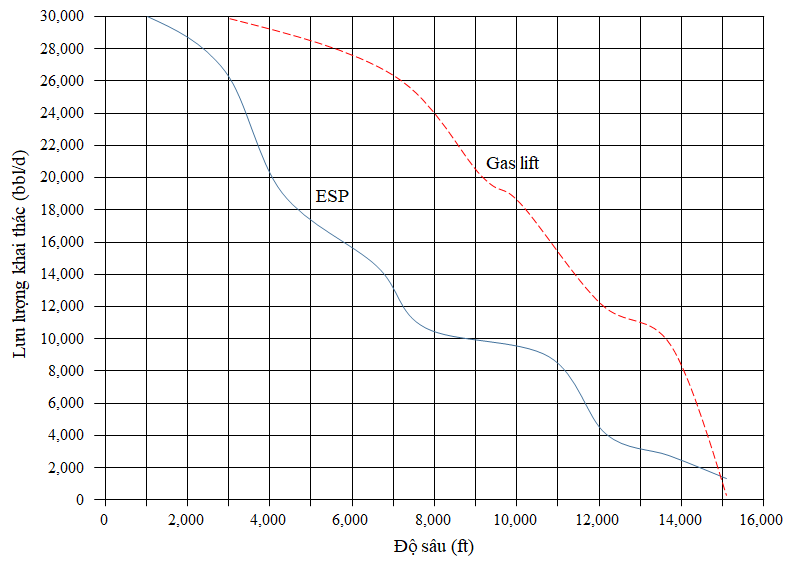
\includegraphics[scale=0.6]{fig/rate-vs-depth.png}
		\caption{Lưu lượng khai thác tối đa theo độ sâu}
		\label{fig:rate-vs-depth}
	\end{figure}

\subsubsection{Ưu điểm và hạn chế}

Một vài ưu điểm của bơm điện li tâm chìm có thể kể đến như sau:
	\begin{itemize}
		\item Thích hợp với khai thác lưu lượng lớn,
		\item Hiệu suất cao,
		\item Sử dụng tốt trong giếng khoan định hướng,
		\item Có thể sử dụng trong điều kiện khu dân cư,
		\item Thích hợp với hoạt động khai thác trên biển,
		\item Dễ dàng sử lý ăn mòn và lắng đọng.
	\end{itemize}
ESP cũng có một vài hạn chế:
	\begin{itemize}
		\item Phụ thuộc vào nguồn cung cấp năng lượng,
		\item Cần được vận hành trong điều kiện ổn định,
		\item Dễ bị ảnh hưởng bởi cát hay các vật chất gây ăn mòn,
		\item Quá trình sửa chửa khó khăn,
		\item Bị hạn chế trong vùng có nhiệt độ cao,
		\item Hiệu suất thấp đối với dầu có độ nhớt cao,
		\item Chi phí lắp đặt cao.\\
	\end{itemize}

\subsection{Gas lift}
Gas lift là phương pháp bơm ép khí vào cột lưu chất trong giếng để lưu chất có thể dễ dàng được khai thác hơn. Hệ thống bề mặt cơ bản cho phương pháp gas lift được thể hiện như trong Hình \ref{fig:gas-lift-system}. Hầu hết khí được sử dụng trong bơm ép là khí tự nhiên có đặc tính trơ, được bơm ép vào trong tubing tại những vị trí đã được thiết kế trước, dựa trên ba nguyên lý chủ yếu: giảm tỉ trọng hỗn hợp lưu chất, năng lượng giản nở của khí và thay thế vị trí. Từ đó dòng lưu chất tại đáy giếng có thể tiếp tục được đưa lên bề mặt và giếng bắt đầu được khai thác trở lại hoặc nâng cao năng suất khai thác. Có thể chia gas lift thành hai loại là gas lift định kì và gas lift liên tục.

	\begin{figure}[h]
		\centering
		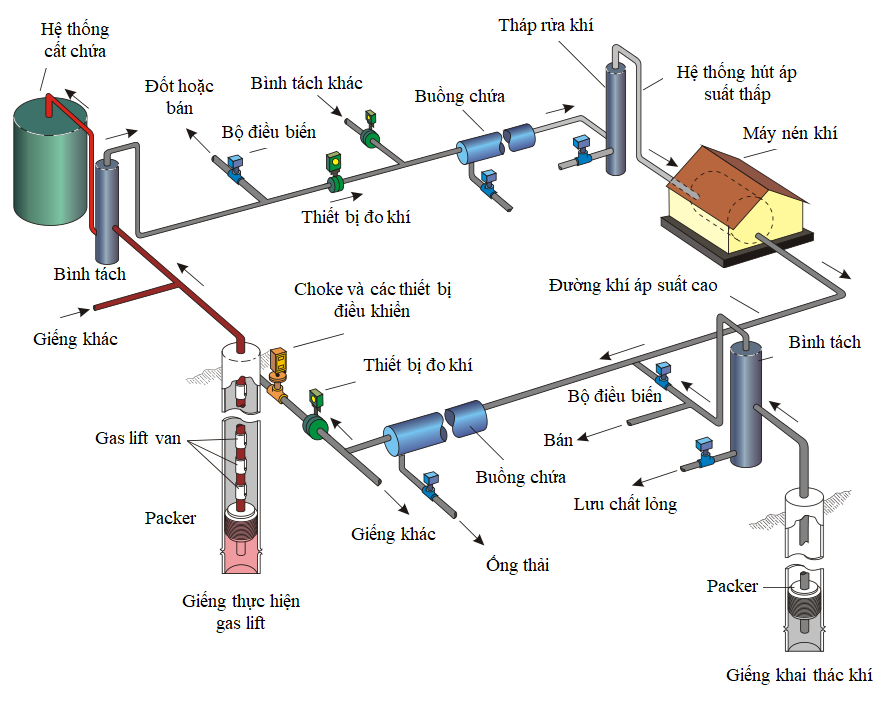
\includegraphics[scale=.6]{fig/gas-lift-system.png}
		\caption{Hệ thống bơm ép gas lift (bề mặt)}
		\label{fig:gas-lift-system}
	\end{figure}

Đối với gas lift liên tục, dòng khí được bơm liên tục có kiểm soát vào trong tubing trong khi gas lift định kì sẽ thực hiện bơm khí theo chu kì nhất định khi lưu chất trong tubing có xu hướng tích tụ về đáy giếng. Sơ đồ lắp đặt một giếng khai thác sử dụng gas lift như Hình \ref{fig:continuous-gas-lift}.

Trong đó, đối với gas lift liên tục van thấp nhất sẽ được mở liên tục để thực hiện bơm ép khí, các van còn lại được vận hành tùy vào mục đích của người vận hành. Đối với gas lift định kì, các van sẽ được mở tùy theo thời gian bơm ép định kì đã lên theo kế hoạch và đóng trong những khoảng thời gian khác. Thông thường trong thời gian bơm ép van số 5 (theo sơ đồ Hình \ref{fig:continuous-gas-lift}) sẽ được mở trước tiên, các van khác được vận hành tùy theo mục đích.

Lưu lượng khí bơm ép cho mỗi giếng được phân chia tùy thuộc vào đặc tính của giếng đó. Trong phạm vi của luận án, tác giả sẽ đi vào xây dựng mô hình phân phối lưu lượng khí cho từng giếng theo cụm giếng chung hệ thống ống góp (manifold). Mô hình sẽ không phân biệt phương pháp gas lift liên tục hay định kì, chỉ đưa ra lưu lượng khí bơm ép cho mỗi giếng dưới điều kiện tổng lượng khí bơm ép xác định để đạt được lưu lượng dầu tối đa trong điều kiện bình tách có thể chịu được.

	\begin{figure}[h]
		\centering
		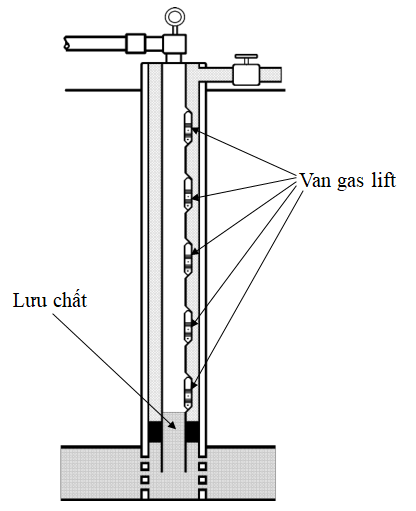
\includegraphics[scale=0.7]{fig/continuous-gas-lift.png}
		\caption{Sơ đồ giếng khai thác với gas lift}
		\label{fig:continuous-gas-lift}
	\end{figure}

\subsubsection{Ứng dụng}
Lần đầu tiên gas lift được đưa vào trong khai thác năm 1846 tại Mĩ, tuy nhiên để sử dụng khai thác nước là chủ yếu. Đến năm 1930 gas lift mới thực sự được đưa vào ứng dụng trong ngành công nghiệp dầu khí cùng với sự ra đời của các mẫu van gas lift khác nhau. Vào những năm này gas lift được sử dụng do hai nguyên chính:
	\begin{itemize}
		\item Tăng mạnh lưu lượng khai thác trong khi năng lượng vỉa bắt đầu suy kiệt,
		\item Đem lại nhiều lợi ích kinh tế khi lượng khí bơm ép sau sử dụng có thể được tách và sử dụng lại, ít bị thất thoát trong quá trình sử dụng.
	\end{itemize}
Trong ngành công nghiệp dầu khí hiện đại, gas lift có những ứng dụng chính như sau:
	\begin{itemize}
		\item Đưa giếng trở lại khai thác sau khi đã kết thúc giai đoạn khai thác tự nhiên,
		\item Tăng lưu lượng khai thác,
		\item Loại bỏ thành phần lỏng trong các giếng khai thác khí,
		\item Xử lý những giếng lắng đọng cát trong giai đoạn bắn mở vỉa,
		\item Khai thác nước cho quá trình bơm ép nước.\\
	\end{itemize}

\subsubsection{Ưu điểm và hạn chế}
Gas lift được xem là một trong những phương pháp phổ biến nhất trong các phương pháp khai thác nhân tạo, phù hợp cho những giếng có độ sâu lớn mà những phương pháp khác không thể thực hiện được. Một số ưu điểm chính có thể kể đến như sau:

Gas lift liên tục:
	\begin{itemize}
		\item Tận dụng tối đa lợi ích do nguồn khí đem lại,
		\item Khai thác lưu lượng lớn,
		\item Thiết bị phổ biến,
		\item Sử dụng được cho giếng có nhiều cát,
		\item Có thể thu hồi van bằng tubing hay dây cáp.
	\end{itemize}
Gas lift định kì:
	\begin{itemize}
		\item Sử dụng được ở điều kiện áp suất dòng vào thấp hơn so với gas lift liên tục,
		\item Thiết bị phổ biến,
		\item Có thể thu hồi van bằng tubing hay dây cáp.
	\end{itemize}

Đồng thời gas lift cũng mang một vài hạn chế như:

Gas lift liên tục:
	\begin{itemize}
		\item Cần nguồn cung cấp khí ổn định,
		\item Không thể triển khai đối với giếng có áp suất quá thấp hoặc có thể nhưng lưu lượng khai thác không khả quan.
	\end{itemize}
Gas lift định kì:
	\begin{itemize}
		\item Không thể cho dòng khai thác lưu lượng lớn,
		\item Có thể gây ra hiệu ứng vọt xung trên bề mặt (surge),
		\item Cần nguồn cung cấp khí ổn định.
	\end{itemize}
Ngoài ra, chi phí ban đầu để triển khai thực hiện gas lift khá cao, quá trình bảo trì và vận hành không dễ dàng.\\

\subsection{Một số phương pháp khác}
Một số phương pháp khai thác nhân tạo khác có thể kể đến như bơm cần, bơm thủy lực hay bơm trục vít. Tuy nhiên, hiện tại các phương pháp không còn được sử dụng phổ biến như hai phương pháp bơm điện li tâm chìm và gas lift. Ưu, nhược điểm của các phương pháp này có thể được kể đến như sau:

Bơm cần (sucker-rod pump)

\begin{table}[h]
\centering
\begin{tabularx}{\textwidth}{@{}XX@{}}
 \multicolumn{1}{c}{Ưu điểm} & \multicolumn{1}{c}{Hạn chế} \\
 \textbullet\ \hspace{0.5cm} Hiệu suất khá cao & \textbullet\ \hspace{0.5cm} Lưu lượng khai thác hạn chế \\
 \textbullet\ \hspace{0.5cm} Chi phí thấp &  \\
 \textbullet\ \hspace{0.5cm} Giảm thiểu ăn mòn &  \\
 \textbullet\ \hspace{0.5cm} Linh hoạt &  \\
 \textbullet\ \hspace{0.5cm} Dễ dàng triển khai cứu hộ và bảo trì & \\
\end{tabularx}
\end{table}

\newpage

Bơm trục vít (progressive cavity pump)

\begin{table}[h]
\centering
\begin{tabularx}{\textwidth}{@{}XX@{}}
 \multicolumn{1}{c}{Ưu điểm} & \multicolumn{1}{c}{Hạn chế} \\
 \textbullet\ \hspace{0.5cm} Hiệu suất khá cao & \textbullet\ \hspace{0.5cm} Bị giới hạn bởi độ sâu giếng \\
 \textbullet\ \hspace{0.5cm} Chi phí đầu tư và bảo trì thấp &  \\
 \textbullet\ \hspace{0.5cm} Ít tiêu tốn năng lượng &  \\
 \textbullet\ \hspace{0.5cm} Có khả năng bơm dầu nặng &  \\
 \textbullet\ \hspace{0.5cm} Dễ dàng triển khai lắp đặt & \\
\end{tabularx}
\end{table}

Bơm thủy lực (subsurface hydraulic pump)

\begin{table}[h]
\centering
\begin{tabularx}{\textwidth}{@{}XX@{}}
 \multicolumn{1}{c}{Ưu điểm} & \multicolumn{1}{c}{Hạn chế} \\
 \textbullet\ \hspace{0.5cm} Linh hoạt trong khai thác đa tầng & \textbullet\ \hspace{0.5cm} Chi phí đầu tư ban đầu cao \\
 \textbullet\ \hspace{0.5cm} Có thể cho lưu lượng khai thác lớn & \textbullet\ \hspace{0.5cm} Vận hành phức tạp \\
 \textbullet\ \hspace{0.5cm} Tần suất bảo trì thấp & \textbullet\ \hspace{0.5cm} Hiệu quả kinh tế cao chỉ khi khai thác đa tầng, đa giếng \\
 \textbullet\ \hspace{0.5cm} Độ sâu khai thác lớn (bơm piston) & \textbullet\ \hspace{0.5cm} Quá trình bảo trì khó khăn \\
\end{tabularx}
\end{table}

\section{Đường cong đặc tính gas lift}
Mục tiếp chính khi sử dụng phương pháp gas lift chính là thu được lưu lượng dầu tối đa với lưu lượng gas lift tối ưu nhất. Mối quan hệ giữa hai đại lượng này được thể hiện thông qua đường cong đặc tính gas lift hay Gas Lift Performance Curve (GLPC)\nomenclature{GLPC}{Gas Lift Performance Curve}. Lưu lượng khí bơm ép tối ưu rất quan trọng, bơm dư hoặc thiếu khí đều làm giảm lưu lượng khai thác đồng thời tăng chi phí bơm ép. Mô hình phân phối lưu lượng khí sẽ được xây dựng dựa trên các tính chất của GLPC cho một giếng khai thác. Dòng chảy trong vỉa được giải sử chỉ bao gồm một pha lỏng, trong tubing sẽ là hai pha lỏng - khí, các điều kiện vật lý để tồn tại GLPC là duy nhất.\\

\subsection{Đường cong đặc tính và bài toán tối ưu}\label{glpc-opt-problem}
Đối với một giếng khai thác bắt đầu thực hiện gas lift, sản phẩm khai thác sẽ bao gồm các lưu chất vỉa (dầu, nước) và khí được bơm ép vào trong tubing. Khi đó lưu lượng khai thác có thể được biểu diễn bằng một hàm phụ thuộc vào lưu lượng khí bơm ép:
	\begin{equation}\label{eqn:GLPC}
		q_l = \varphi(q_g)
	\end{equation}
Với:\\
\hspace*{1cm}$q_g$ là lưu lượng khí bơm ép\nomenclature{$q_g$}{Lưu lượng khí bơm ép (MSCF/d)}\\
\hspace*{1cm}$q_l$ là lưu lượng khai thác.\nomenclature{$q_l$}{Lưu lượng khai thác (lỏng) (STB/d)}

Nếu hàm số $\varphi(q_g)$ tồn tại, đồ thị biểu diễn đường cong hàm số \ref{eqn:GLPC} chính là đường đặc tính gas lift (Hình \ref{fig:glpc}). Để \ref{eqn:GLPC} tồn tại $q_g$ phải thỏa mãn điều kiện $0 \leq q_g \leq Q_{gav}$\nomenclature{$Q_{gav}$}{Tổng lượng khí có sẵn} với $Q_{gav}$ là tổng lượng khí có sẵn.

	\begin{figure}[h]
		\centering
		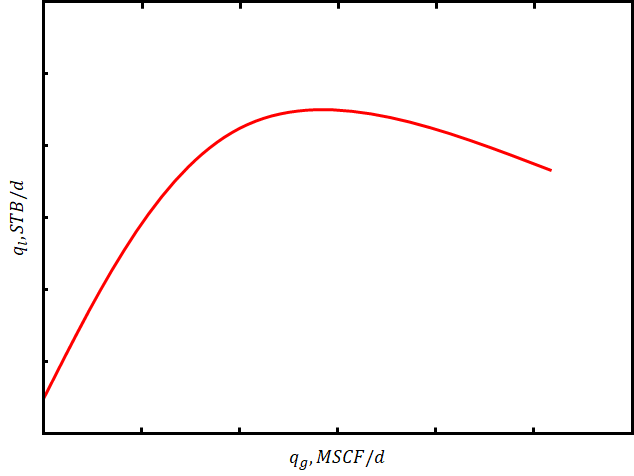
\includegraphics[scale=.6]{fig/glpc.png}
		\caption{Đường đặc tính gas lift}
		\label{fig:glpc}
	\end{figure}

Sử dụng các đặc tính khai thác của mỗi giếng lưu lượng dầu được tính thông qua phương trình:
	\begin{equation}\label{eqn:qo-vs-ql}
		q_o = (1 - WC) \times q_l
	\end{equation}
Với:\\
\hspace*{1cm}WC là hàm lượng nước trong lưu chất khai thác\nomenclature{WC}{Hàm lượng nước}\\
\hspace*{1cm}$q_o$ là lưu lượng dầu.\nomenclature{$q_o$}{Lưu lượng dầu (STB/d)}

Từ các phương trình \ref{eqn:GLPC} và \ref{eqn:qo-vs-ql} được:
	\begin{equation}\label{eqn:qo-vs-qg}
		q_o = (1 - WC) \times \varphi(q_g)
	\end{equation}
Quá trình tối đa hóa lưu lượng dầu sẽ xoay quanh việc tìm giá trị lớn nhất của phương trình \ref{eqn:qo-vs-qg}:
	\begin{equation}\label{eqn:max-qo}
		Max\sum_{k=1}^Nq_o = Max\sum_{k=1}^N(1 - WC) \times \varphi(q_g)
	\end{equation}
Với N là tổng số giếng trong cụm giếng và k là giếng khai thác.\\

\subsection{Mô hình hình toán học}
Để có thể thực hiện xây dụng mô hình phân phối tối ưu cần đưa bài toán tối ưu như đã nêu ở mục \ref{glpc-opt-problem} trở về dưới dạng tối ưu bằng mô hình toán học. Bắt đầu với phương trình biểu diễn chỉ số năng suất khai thác được suy ra từ định luật Darcy:
	\begin{equation}\label{eqn:darcy-productivity-index}
		J = \dfrac{q_l}{P_r - P_{wf}}
	\end{equation}
Với:\\
\hspace*{1cm}J là chỉ số năng suất\nomenclature{J}{Chỉ số năng suất (STB/d/psi)}\\
\hspace*{1cm}$P_r$ là áp suất vỉa\nomenclature{$P_r$}{Áp suất vỉa}\\
\hspace*{1cm}$P_{wf}$ là áp suất dòng vào tại đáy giếng.\nomenclature{$P_{wf}$}{Áp suất dòng vào tại đáy giếng}

Bằng cách giả sử lưu chất vỉa chỉ tồn tại một pha lỏng (dầu và nước), ta có được:
	\begin{equation}\label{eqn:qo-ql-wc}
		q_l = (1 + WOR) \times q_o = \dfrac{q_o}{1 - WC}
	\end{equation}
Với WOR\nomenclature{WOR}{Tỉ số nước dầu} là tỉ số nước - dầu.

Phương trình dòng chảy cho lưu chất hai pha trong tubing được biểu diển từ \textit{phương trình cân bằng năng lượng}:
	\begin{equation}\label{eqn:energy-balance-equation}
		\dfrac{dP}{dz} = \dfrac{g}{g_c}\overline{\rho}sin(\theta) + \dfrac{f\overline{\rho}u_m^2}{2g_cD} + \dfrac{\overline{\rho}}{2g_c}\dfrac{D}{dz}u_m^2
	\end{equation}
Với điều kiện ban đầu:
	\begin{equation}\label{eqn:initial-cons}
		P(0) = P_{wh}
	\end{equation}
Trong đó:\\
\hspace*{1cm}P: Áp suất mất mát (psi)\nomenclature{P}{Áp suất}\\
\hspace*{1cm}z: Chiều sâu giếng khoan (ft)\nomenclature{z}{Chiều sâu giếng khoan}\\
\hspace*{1cm}g: Gia tốc trọng trường $(\text{ft}/\text{s}^2)$\\
\hspace*{1cm}$g_c$: Hệ số chuyển đổi\\
\hspace*{1cm}$\overline{\rho}$: Tỉ trọng hỗn hợp\nomenclature{$\overline{\rho}$}{Tỉ trọng hỗn hợp}\\
\hspace*{1cm}D: Đường kính tubing (in)\nomenclature{D}{Đường kính tubing (in)}\\
\hspace*{1cm}$f$: Hệ số ma sát\nomenclature{$f$}{Hệ số ma sát}\\
\hspace*{1cm}$u_m$: Vận tốc hỗn hợp (ft/s).\nomenclature{$u_m$}{Vận tốc hỗn hợp (ft/s)}

Các thành phần $\dfrac{g}{g_c}\overline{\rho}sin(\theta)$, $\dfrac{f\overline{\rho}u_m^2}{2g_cD}$ và $\dfrac{\overline{\rho}}{2g_c}\dfrac{d}{dz}u_m^2$ trong phương trình \ref{eqn:energy-balance-equation} tương ứng là tổn hao áp suất do thế năng, ma sát và động năng. Đối với giếng thẳng đứng $sin(\theta) = 1$ do đó thành phần thế năng trở thành $\dfrac{g}{g_c}\overline{\rho}$, thành phần động năng tương đối nhỏ có thể bỏ qua. $\overline{\rho}$ được miêu tả bằng phương trình:
	\begin{equation}\label{eqn:mixture-density}
		\overline{\rho} = H_g\rho_g + (1 - H_g)\rho_l
	\end{equation}
Tỉ trọng của khí $\rho_g$ phụ thuộc áp suất P theo công thức:
	\begin{equation}\label{eqn:gas-density}
		\rho_g = 28.97\dfrac{\gamma_gP}{ZRT}
	\end{equation}
Với:\\
\hspace*{1cm}Z: Hệ số lệch khí\\
\hspace*{1cm}R: Hằng số khí phổ\\
\hspace*{1cm}T: Nhiệt độ trung bình trong tubing.

Tỉ số thể tích khí trong hỗn hợp $H_g$ được tính theo mô hình Zuber-Findlay:
	\begin{equation}\label{eqn:gas-holdup}
		H_g = \dfrac{u_{sg}}{C_ou_m + U_d}
	\end{equation}
Với:\\
\hspace*{1cm}$u_{sg}$: Tốc độ trượt của khí\\
\hspace*{1cm}$C_o$: Hệ số phân tán\\
\hspace*{1cm}$U_d$: Tốc độ trôi.

Tốc độ của hỗn hợp lưu chất được tính toán từ tốc độ trượt của pha khí và pha lỏng theo các công thức:
	\begin{equation}\label{eqn:mixture-velocity}
		u_m = u_{sl} + u_{sg}
	\end{equation}
	\begin{equation}\label{eqn:usg-usl}
		u_{sl} = \dfrac{q_l}{A},\hspace*{1cm} u_{sg} = \dfrac{ZP_{sc}T}{T_{sc}P}\dfrac{q_g}{A},\hspace*{1cm} A = \pi\dfrac{D^2}{4}
	\end{equation}
Với:\\
\hspace*{1cm}$u_{sl}$: Tốc độ trượt của pha lỏng ($\text{ft}/\text{s}^2$)\\
\hspace*{1cm}$u_{sg}$: Tốc độ trượt của pha khí ($\text{ft}/\text{s}^2$)\\
\hspace*{1cm}A: Tiết diện của tubing.

\section{Trí tuệ nhân tạo}
Trí tuệ nhân tạo hay Artificial Intelligence (AI)\nomenclature{AI}{Artificial Intelligence} là một phương pháp sử dụng sức mạnh của máy tính để giải những bài toán khó trong đó có bài toán tối ưu hóa. Để có thể giải được những bài toán tối ưu hóa hiện đại, những kĩ thuật cổ điển không còn thích hợp; tuy nhiên, khi không gian tối ưu lớn đi kèm các ràng buộc đặc biệt cần phải sử dụng những kĩ thuật thích hợp. \textit{Giải thuật di truyền} và \textit{mạng thần kinh nhân tạo} (hay mạng neural nhân tạo, ANN)\nomenclature{ANN}{mạng thần kinh nhân tạo} là hai trong những kĩ thuật đó.\\

\subsection{Giải thuật di truyền}
\subsubsection{Nguyên lý giải thuật}
Giải thuật di truyền (Genetic Algorithms, GA)\nomenclature{GA}{Giải thuật di truyền}; thuật ngữ ``giải thuật'' ở đây chính là các thuật toán để giải quyết một vấn đề; được mô phỏng dựa trên các hiện tượng sinh học tự nhiên: \textit{kế thừa} và \textit{đấu tranh sinh tồn} để thực hiện cải tiến, khảo sát không gian của lời giải. Khái niệm kế thừa và đấu tranh sinh tồn có thể được giải thích như sau:

Giả sử có một quần thể các cá thể loài chồn, bao gồm những cá thể vượt trội có sự linh hoạt, nhạy bén cao, khỏe mạnh và những cá thể yếu ớt không đủ linh hoạt nhạy bén. Những cá thể vượt trội có xác suất sinh tồn trong môi trường tự nhiên cao hơn các cá thể yếu ớt, dĩ nhiên một số cá thể yếu ớt cũng có thể sống được nhờ may mắn đó chính là đấu tranh sinh tồn. Đến một giai đoạn nào đó các cá thể chồn còn lại bắt đầu sinh sản, thế hệ các chú chồn tiếp theo sẽ được kế thừa các đặc tính di truyền của các con bố và mẹ, tất nhiên là có một số con mang đặc tính của những con yếu ớt còn sót lại; điều này chính là kế thừa. Đôi khi sẽ có thêm những cá thể đột biến do mang đặc tính di truyền từ một các thể khác lạc vào quần thể chồn này, cá thể đột biến này có thể tốt hoặc xấu. Do đó, thế hệ sau luôn mang một xác suất cao cho ra những cá thể tốt hơn thế hệ trước. Tất nhiên quần thể những loài thú săn chồn cũng mang đặc tính kế thừa và đấu tranh này.

Quá trình tìm kiếm ngiệm của bài toán tối ưu bằng giải thuật di truyên cũng thực hiện các bước tương tự với quá trình đấu tranh sinh tồn của quần thể chồn. 

Giải thuật di truyền sử dụng một số thuật ngữ được lấy từ di truyền học như: cá thể, quần thể, nhiễm sắc thể, kiểu gen. Một cá thể cũng là một nhiễm sắc thể đươc cấu tạo từ các gen, mỗi gen mang một đặc trưng khác nhau. Trong toán học một nghiệm của phương trình chính là nhiễm sắc thể, một thành phần trong nghiệm chính là một gen, tập hợp của một số các cặp số có thể trở thành nghiệm của phương trình chính là quần thể. Ví dụ tìm cực trị của hàm số hai biến $x$, $y$ sau:
	\begin{equation}\label{eqn:ex-genetic}
		f(x, y) = x^2y + y^2x
	\end{equation}
Giả sử $A = (x_1, y_1)$ chính là một nghiệm của \ref{eqn:ex-genetic}, như vậy $A$ sẽ là một nhiễm sắc thể; $x_1$, $y_1$ là các gen của nhiễm sắc thể $A$; tập hợp $A_1 \to A_N$ là một quần thể chứa các nhiễm sắc thể có thể là nghiệm của \ref{eqn:ex-genetic} với số lượng cá thể $N$ tùy thuộc vào sự lựa chọn của người giải.\\

\subsubsection{Thuật toán di truyền}
Một thuật toán di truyền để giải bất kì một bài toán cụ thể nào phải bao gồm năm điểm sau:
	\begin{itemize}
		\item Cách biểu diễn di truyền cho lời giải của bài toán,
		\item Các khởi tạo quần thể ban đầu,
		\item Một hàm lượng giá đóng vai trò là môi trường, đánh giá các lời giải theo mức độ ``thích nghi'' của chúng,
		\item Các phép toán di truyền,
		\item Các tham số khởi tạo (kích thước quần thể, xác suất áp dụng các phép toán di truyền, hoán đổi...).
	\end{itemize}
Cụ thể thuật toán di truyền được diễn giải thông qua các phép sau:

\textit{a. Phép chọn}

Phép chọn là quá trình loại bỏ các cá thể xấu trong quần thể chỉ giữ lại những các thể tốt dựa trên độ thích nghi của mỗi cá thể. Độ thích nghi là một hàm gán một giá trị thực cho các cá thể trong quần thể. Phép chọn có thể được mô phỏng như sau:
	\begin{itemize}
		\item Đánh giá độ thích nghi của từng cá thể trong quần thể hiện hành,
		\item Sắp xếp quần thể theo độ thích nghi giảm dần,
		\item Loại bỏ các cá thể cuối dãy, chỉ giữ lại $n$ cá thể tốt nhất.
	\end{itemize}

\textit{b. Phép lai}

Phép lai là quá trình hình thành nhiễm sắc thể mới trên cơ sở các nhiễm sắc thể bố-mẹ, bằng cách ghép một hay nhiều đoạn gen của hai (hay nhiều) nhiễm sắc thể bố-mẹ với nhau. Phép lai xảy ra với xác suất $p_c$, có thể mô phỏng như sau:
	\begin{itemize}
		\item Chọn ngẫu nhiên hai (hay nhiều) cá thể bất kỳ trong quần thể. Giả sử các nhiễm sắc thể bố-mẹ đều có $m$ gen,
		\item Tạo ngẫu nhiên một số tự nhiên trong đoạn $[1, m-1]$ (điểm lai). Điểm lai chia các chuỗi bố-mẹ dài $m$ thành hai nhóm chuỗi con dài $m_1$, $m_2$. Hai chuỗi nhiễm sắc thể con mới sẽ là $m_{11} + m_{22}$ và $m_{12} + m_{21}$.
	\end{itemize}

\textit{c. Phép đột biến}

Đột biến là hiện tượng cá thể con mang một số tính trạng không có trong mã gen di truyền của bố-mẹ. Phép đột biến xảy ra với xác suất $p_m$ nhỏ hơn rất nhiều so với xác suất lai $p_c$. Phép đột biến có thể mô phỏng như sau:
	\begin{itemize}
		\item Chọn ngẫu nhiên một cá thể bất kì bố-mẹ trong quần thể,
		\item Tạo ngẫu nhiên một số tự nhiên $k$ trong đoạn $[1, m]$,
		\item Thay đổi gen thứ $k$ và trả cá thể này về quần thể để tham gia quá trình tiến hóa tiếp theo.
	\end{itemize}

\textit{d. Phép tái sinh}

Phép tái sinh là quá trình trong đó các cá thể được sao chép trên cơ sở độ thích nghi của nó. Quá trình này có thể được mô tả như sau:
	\begin{itemize}
		\item Tính độ thích nghi của từng cá thể trong quần thể hiện hành, lập bảng cộng dồn các giá trị thích nghi (theo số thứ tự cho từng cá thể). Giả sử quần thể có $n$ cá thể. Gọi độ thích nghi của cá thể thứ $i$ là $F_i$, tổng cộng dồn thứ $i$ là $F_{ti}$, tổng độ thích nghi của toàn quần thể là $F_{m}$,
		\item Tạo một số ngẫu nhiên $F$ trong đoạn $[0, F_m]$,
		\item Chọn cá thể thứ $k$ đầu tiên thỏa $F \geq F_{tk}$ đưa vào quần thể của thế hệ mới.
	\end{itemize}

Sau khi đã thực hiện phép tái sinh, sẽ bắt đầu một vòng lặp mới cho thế hệ mới sinh từ phép chọn cho đến nghiệm hội tụ hoặc chạy hết số vòng lặp được thiết lập. Thuật toán được thể hiện cụ thể theo sơ đồ Hình \ref{fig:genetic-algorithms}. Điều kiện thực hiện ``yes, no'' là nghiệm đã hội tụ hoặc đã chạy hết vòng lặp hay chưa. Tham số đầu vào bao gồm xác suất lai tạo ($p_c$) và đột biến ($p_m$), kích thước quần thể ($N$), thành phần nghiệm của phương trình ($n_{vars}$), hàm lượng giá.

	\begin{figure}[h]
		\centering
		\begin{tikzpicture}[node distance=2cm]
			\node (start) [startstop] {Bắt đầu};
			\node (param) [io, below of=start] {Tham số đầu vào};
			\node (init) [process, below of=param] {Khởi tạo quần thể};
			\node (eval) [decision, below of=init, yshift=-0.5cm] {Đánh giá};
			\node (selection) [process, below of=eval, yshift=-0.3cm] {Lựa chọn};
			\node (crossover) [process, below of=selection, yshift=-0.3cm] {Lai tạo};
			\node (mutation) [process, below of=crossover, yshift=-0.3cm] {Đột biến};
			\node (recreate) [process, below of=mutation, yshift=-0.3cm] {Tái sinh};
			\node (new_pop) [process, right of=recreate, xshift=2.5cm] {Quần thể mới};
			\node (out) [io, below of=recreate] {Kết quả};
			\node (stop) [startstop, left of=eval, xshift=-2cm] {Dừng};

			\draw [arrow] (start) -- (param);
			\draw [arrow] (param) -- (init);
			\draw [arrow] (init) -- (eval);
			\draw [arrow] (eval) -- node[anchor=south] {yes} (stop);
			\draw [arrow] (eval) -- node[anchor=east] {no} (selection);
			\draw [arrow] (selection) -- (crossover);
			\draw [arrow] (crossover) -- (mutation);
			\draw [arrow] (mutation) -- (recreate);
			\draw [arrow] (recreate) -- (new_pop);
			\draw [arrow] (new_pop) |- (eval);
			\draw [arrow] (stop) |- (out);
		\end{tikzpicture}
		\caption{Thuật toán di truyền}
		\label{fig:genetic-algorithms}
	\end{figure}

\clearpage

\subsection{Mạng thần kinh nhân tạo}

\section{Thuật toán tối ưu}

\end{document}